\documentclass[12pt]{article}
\usepackage{amsmath}
\usepackage{epsfig}
\usepackage{lscape}
%\usepackage{rotating}
\usepackage{array}
\topmargin 0in \headheight 0.0in \textheight 9in \textwidth 6.5in
\oddsidemargin 0.1in \evensidemargin 0.1in
\renewcommand{\baselinestretch}{1.6}
\newcommand{\beq}{\begin{equation}}
\newcommand{\eeq}{\end{equation}}
\newcommand{\ie}{\emph{i.e.}}
\newcommand{\eg}{\emph{e.g.}}
\begin{document}

\title{The connection between graph signal processing and eigen vector spatial filtering to analyze imaging data (this specific?)}
\maketitle

\section{Background}

This work is motivated by a desire to account for the complex spatial structure in analysis of imaging data (CT, neuroimaging, etc).

There have been two parallel developments in the literature - explain both and cite the literature.

Graph Signal Processing.  - estimate the network is the focus (infers structure underneath).  But some have applied GSP.  Assume some structure and figure out the auto correlation--get features like 

ESF uses eigen decomposition to model correlation and get better inference on fixed effects.

The purpose of this paper is to draw direct connections between these two parallel developments of [insert] and to apply various approaches from both areas to highlight the advantages of each approach to analyzing imaging data. We conduct analysis using a traditional EFS approach, prediction [outline more], and GSP approaches to estimate a network and use an estimated network to [do what]. We do this on a toy example to clearly exhibit the links between the approaches, on neuroimaging data in aging (BIOAD), and chest (lung) CT in sarcoidosis.

\section{Methods}
\subsection{Eigen vector spatial filtering}
[Cut from Sarah Ryan paper so will need editing but will give you a notational start]. Eigenvector spatial filtering (ESF) is a technique used to model spatially distributed data using a linear combination of spatial eigenvectors \citep{griffith1996spatial}. The spatial eigenvectors are constructed by the eigen-decomposition of a centered spatial covariance function, such as the exponential, gaussian, or spherical.  For the set of unique spatial locations, $S$, let $\mathbf{C}$ be an $(S \times S)$ symmetric spatial covariance function and $\mathbf{M}=I - 11^\prime/S$ be a centering matrix \citep{griffith1996spatial}. Then, $\mathbf{M} \mathbf{C} \mathbf{M}$ is eigen-decomposed into $\mathbf{E}_\textit{full} \mathbf{\Lambda}_\textit{full} \mathbf{E}_\textit{full}^\prime$, where $\mathbf{E}_\textit{full}$ is a square matrix composed of eigenvectors and $\mathbf{\Lambda}_\textit{full}$ is a diagonal matrix whose diagonal elements are the eigenvalues. We note that the choice of $C$ is made without reference to the data through specification of a spatial covariance model and parameters. 

The complete set of eigenvectors, $\mathbf{E}_\textit{full}$, provides all possible distinct map patterns of spatial dependence for the given distance matrix, where the first eigenvector has the largest spatial dependence for the given distance matrix and corresponds to the largest spatial pattern; the second eigenvector, uncorrelated with the first, has the second largest spatial dependence and corresponds to the second largest spatial pattern, and so forth. Here we note that the map is the constructed lung template of voxel locations. This means that $\mathbf{E}_\textit{full}$ represents the spatial dependencies on a lung template and is not dependent on the observed HU on a chest CT.

Often, the complete set of eigenvectors is not necessary to model the spatial pattern in the data. Thus, a subset of $L$ eigenvectors, $\mathbf{E}$, of dimension $(S \times L)$ where $L<<S$, may be selected. Often, only eigenvectors associated with positive eigenvalues, which correspond to positive spatial dependence, are selected since positive spatial correlation is observed naturally \citep{griffith2014spatial, griffith2006spatial, chun2014quality}. Note that the eigenvectors are also directly related to Moran's I, a measure of spatial dependence; for more information, see \cite{murakami2019eigenvector}. 

Despite starting with n spatial maps, one for each subject in our analysis, we register each image to a lung template \citep{ryan2019template}. Thus, the spatial coordinate system is the same across all images, and we are able to construct a single eigenvector matrix $\mathbf{E}$, which comes with considerable computational savings. To illustrate the spatial patterns represented by the spatial eigenvectors in lungs, we have plotted selected eigenvectors associated with positive eigenvalues from a two-dimensional slice of the right lung (Figure \ref{fig:eigenvectors}). This slice is based on the median axial slice from the standard lung template \citep{ryan2019template}, and is comprised of 1578 unique voxels at $3mm^2$ voxel spacing. As shown in Figure \ref{fig:eigenvectors}, the first eigenvector has the largest, most global, spatial structure, with each subsequent eigenvector having smaller scale spatial structures. There were 397 eigenvectors associated with positive spatial correlation in this two-dimensional slice of the lung. We follow existing geostatistical literature \citep{griffith2014spatial, griffith2006spatial, chun2014quality} to model the lung using only eigenvectors associated with positive spatial dependence, as we observe this works well in practice [should we change this?, would require code modification].

% For notational simplicity, we assume no missing data across the scans, resulting in the same eigenvector matrix, $\mathbf{E_i}$, for each scan/subject $i=1, \dots, n$ (E.g. $\mathbf{E}(s) = \mathbf{E_i}(s) \forall i$). In practice, this approach can easily handle missing data, which may occur due to imperfect segmentation and registration, and is allowable in our code.  


\begin{figure}
\centering 
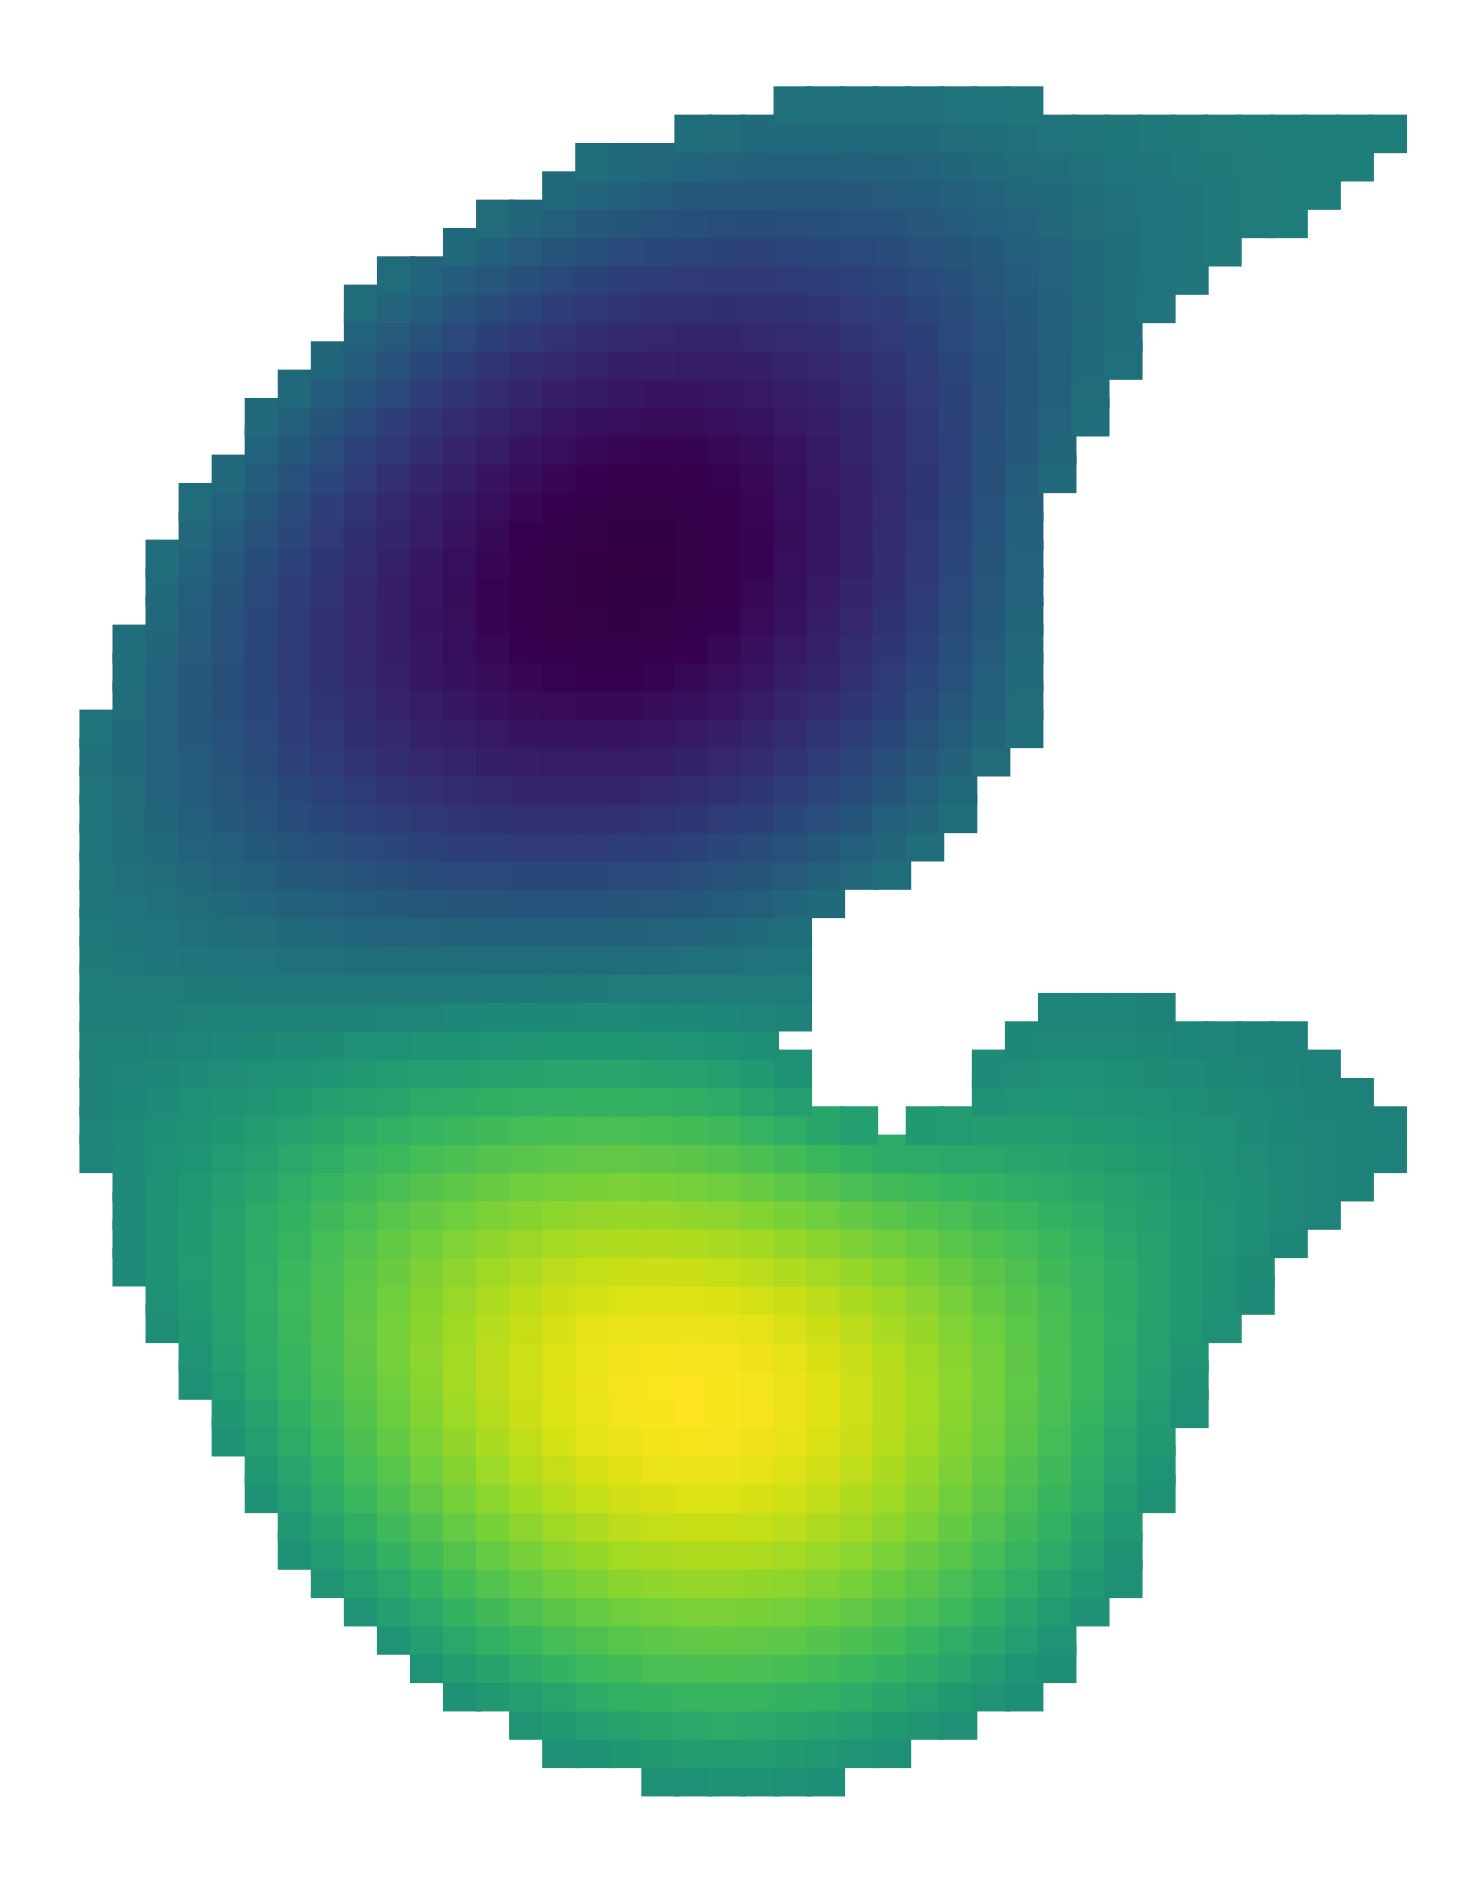
\includegraphics[height=1.5in]{EV1}
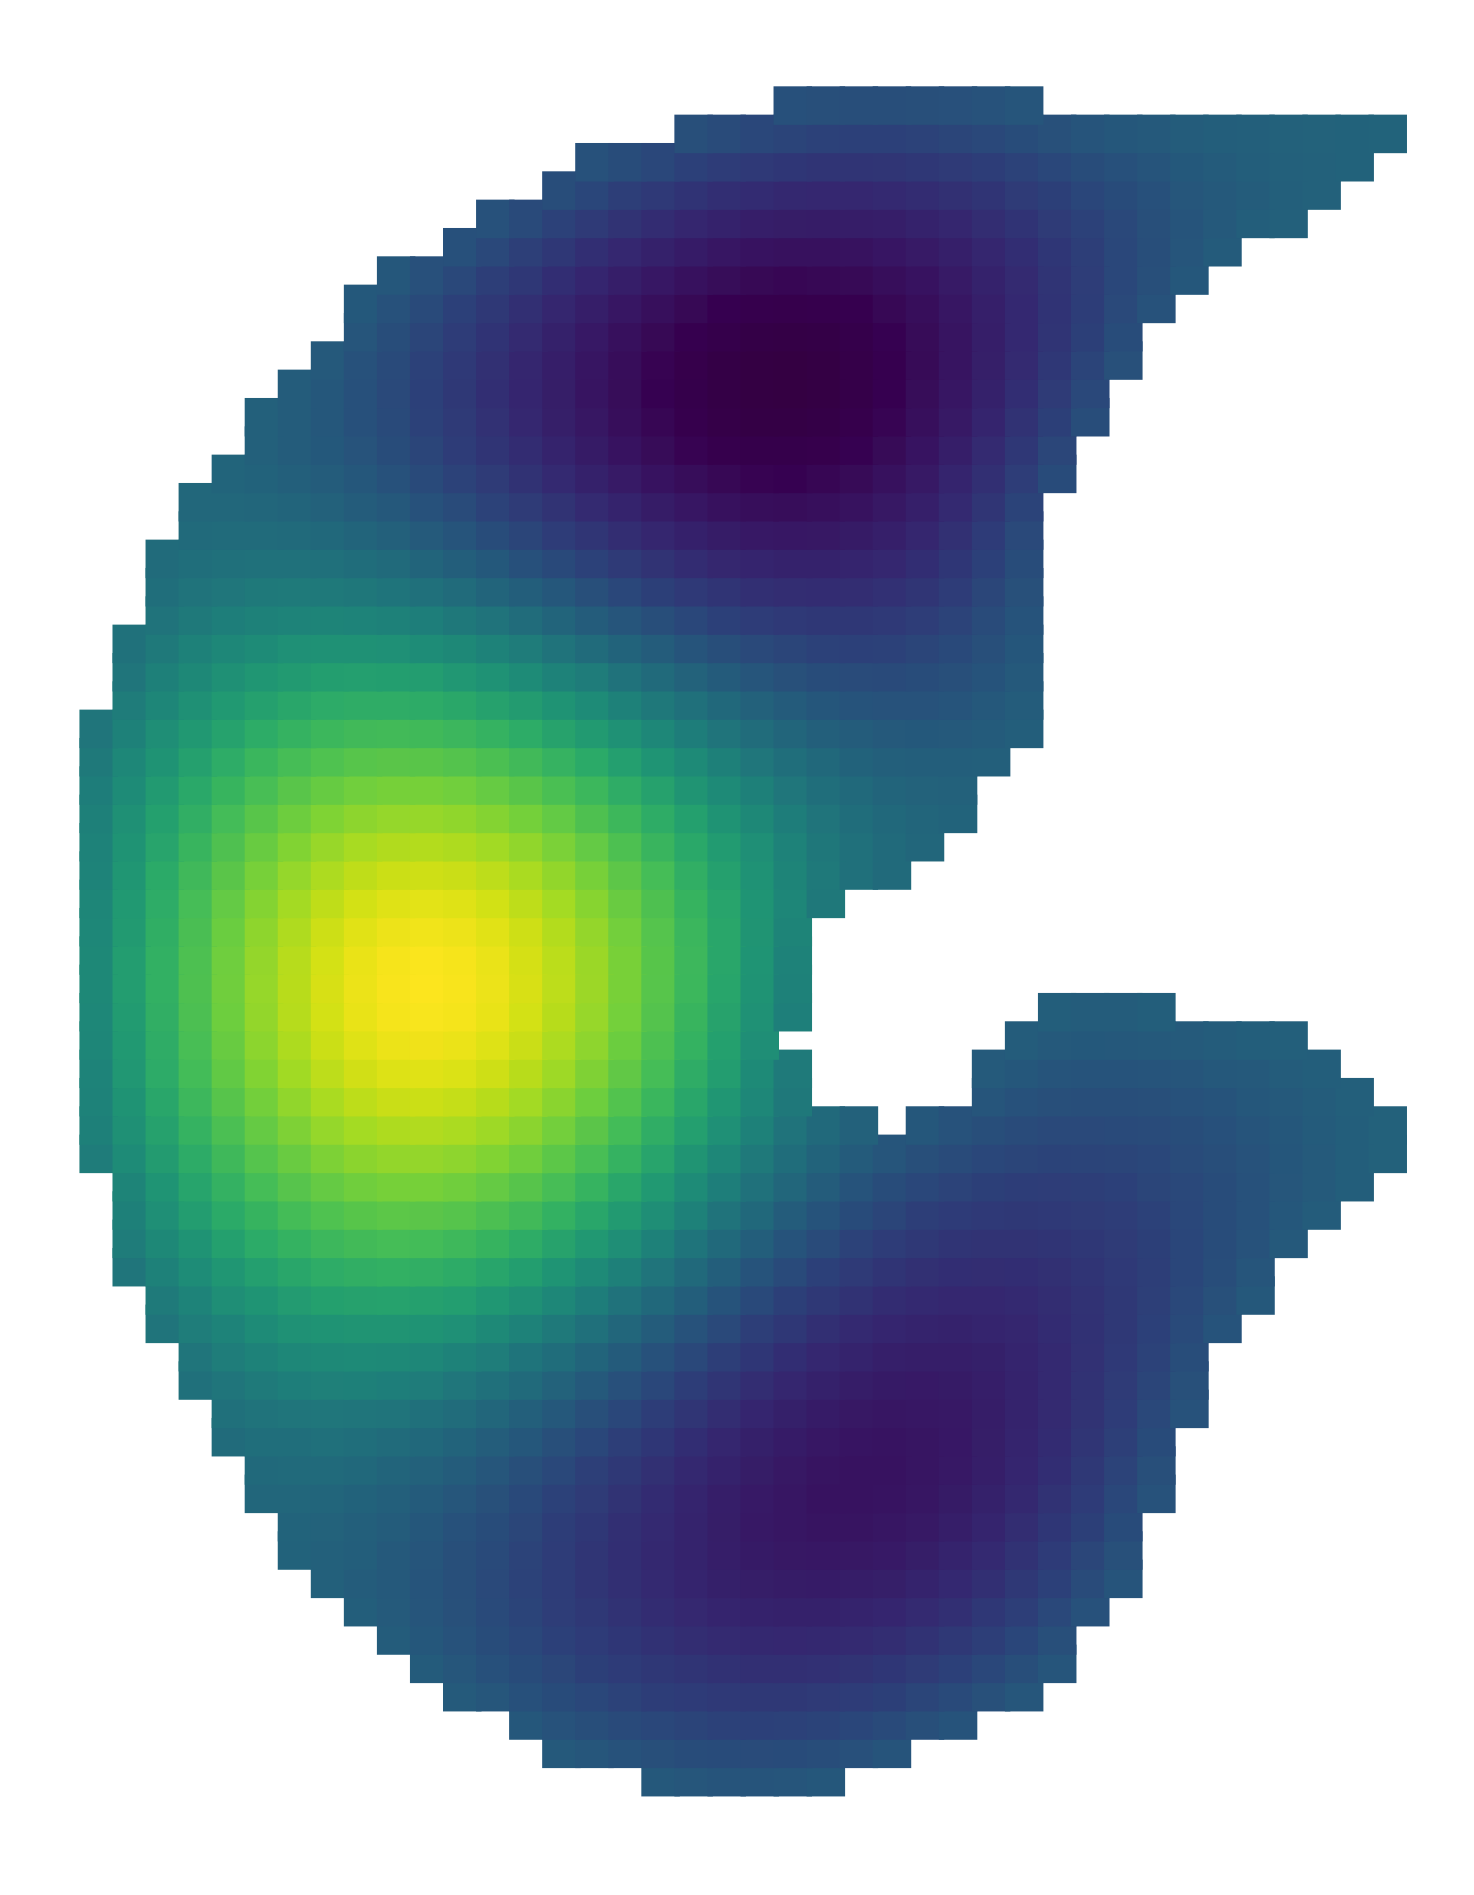
\includegraphics[height=1.5in]{EV2}
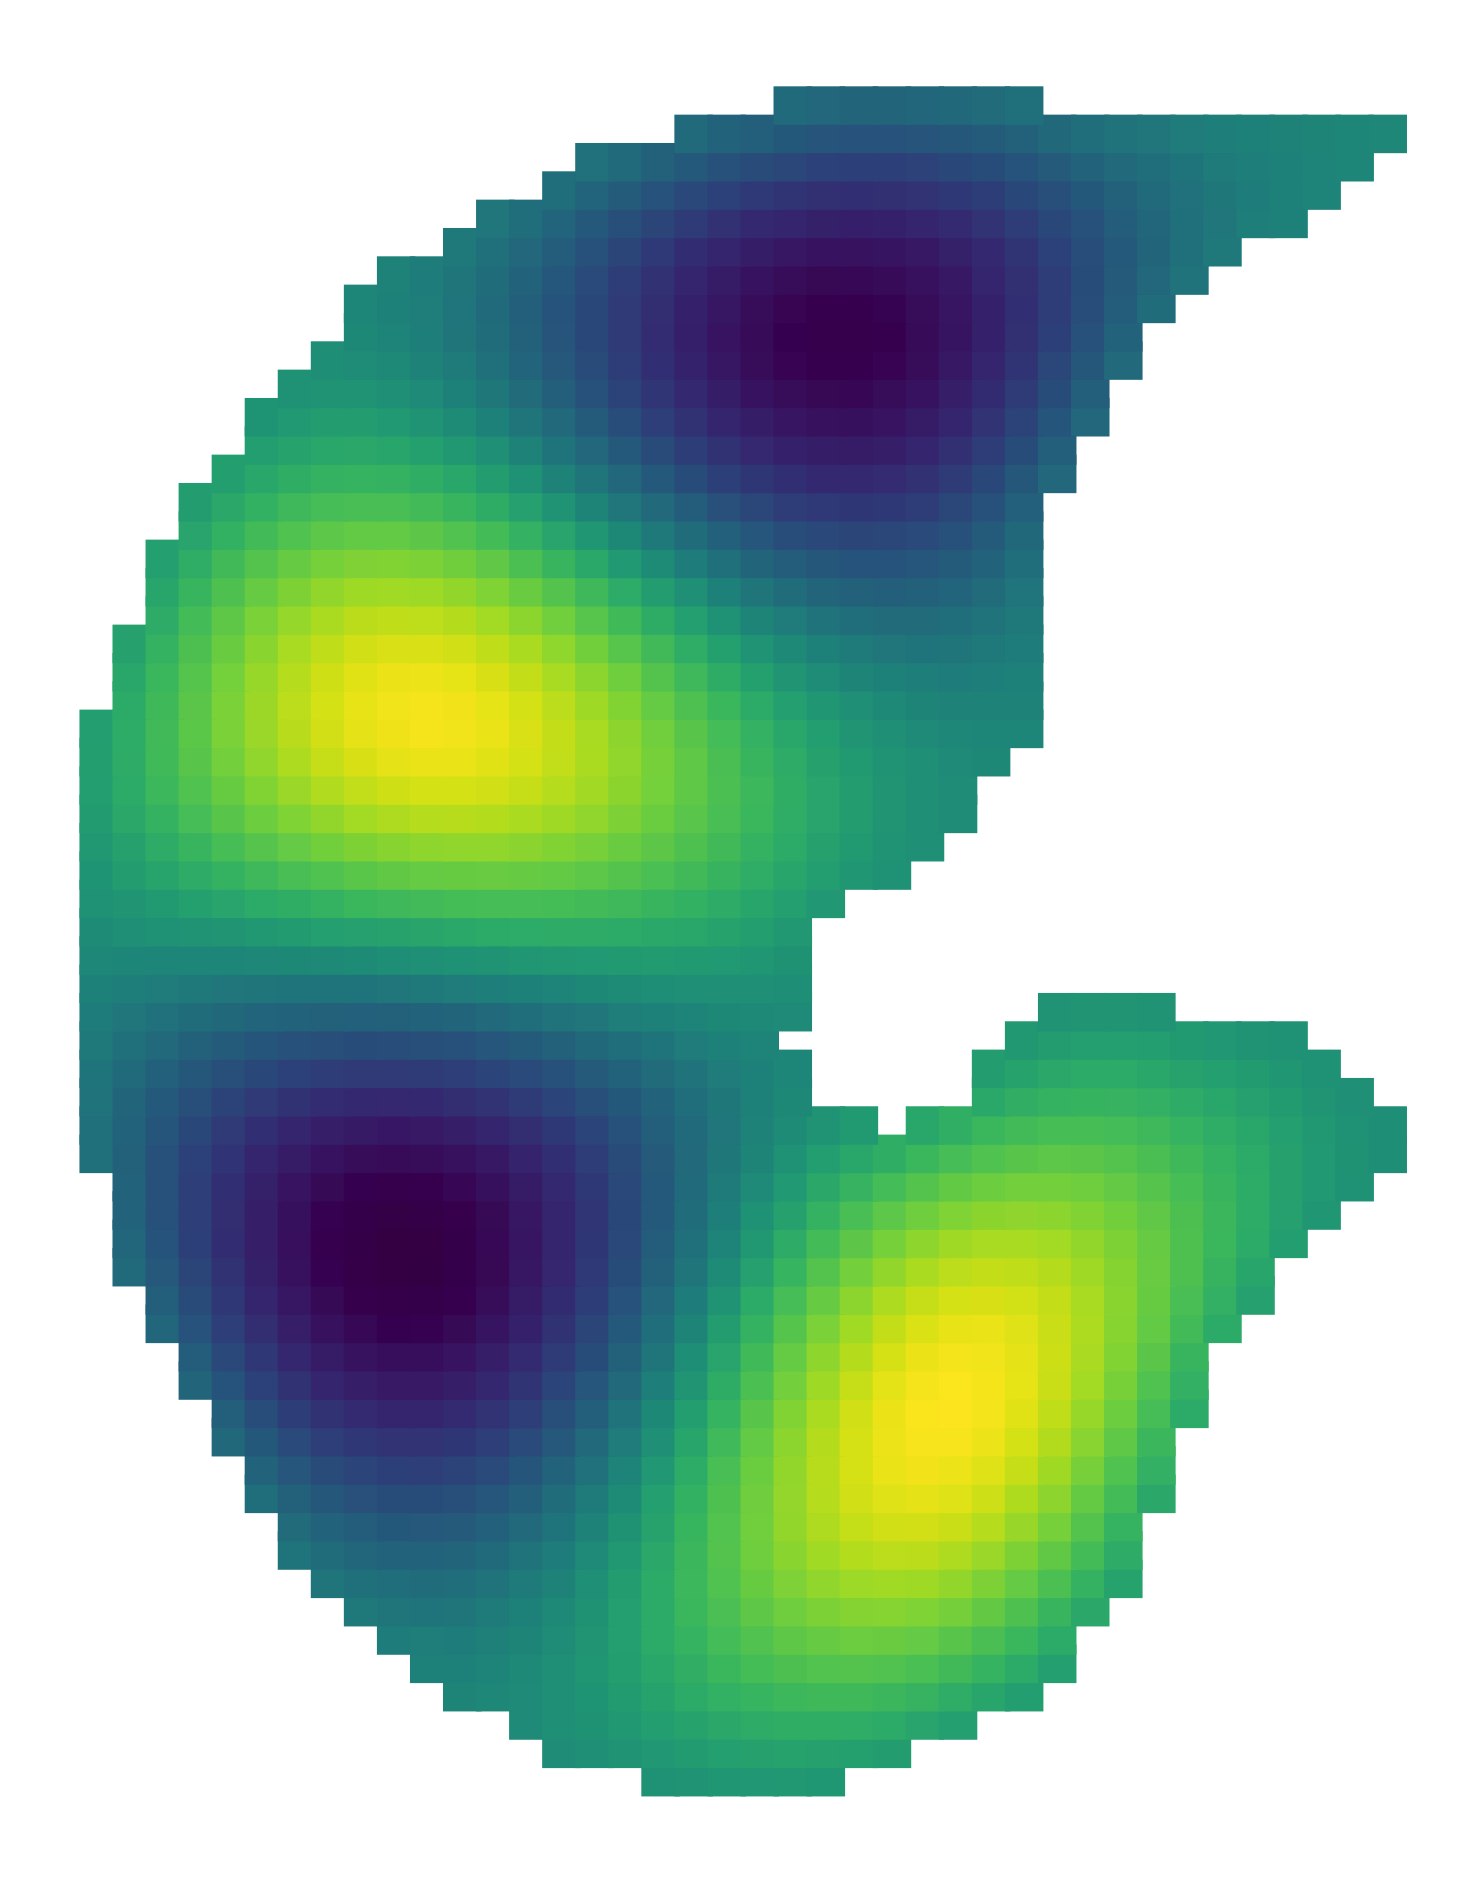
\includegraphics[height=1.5in]{EV3}
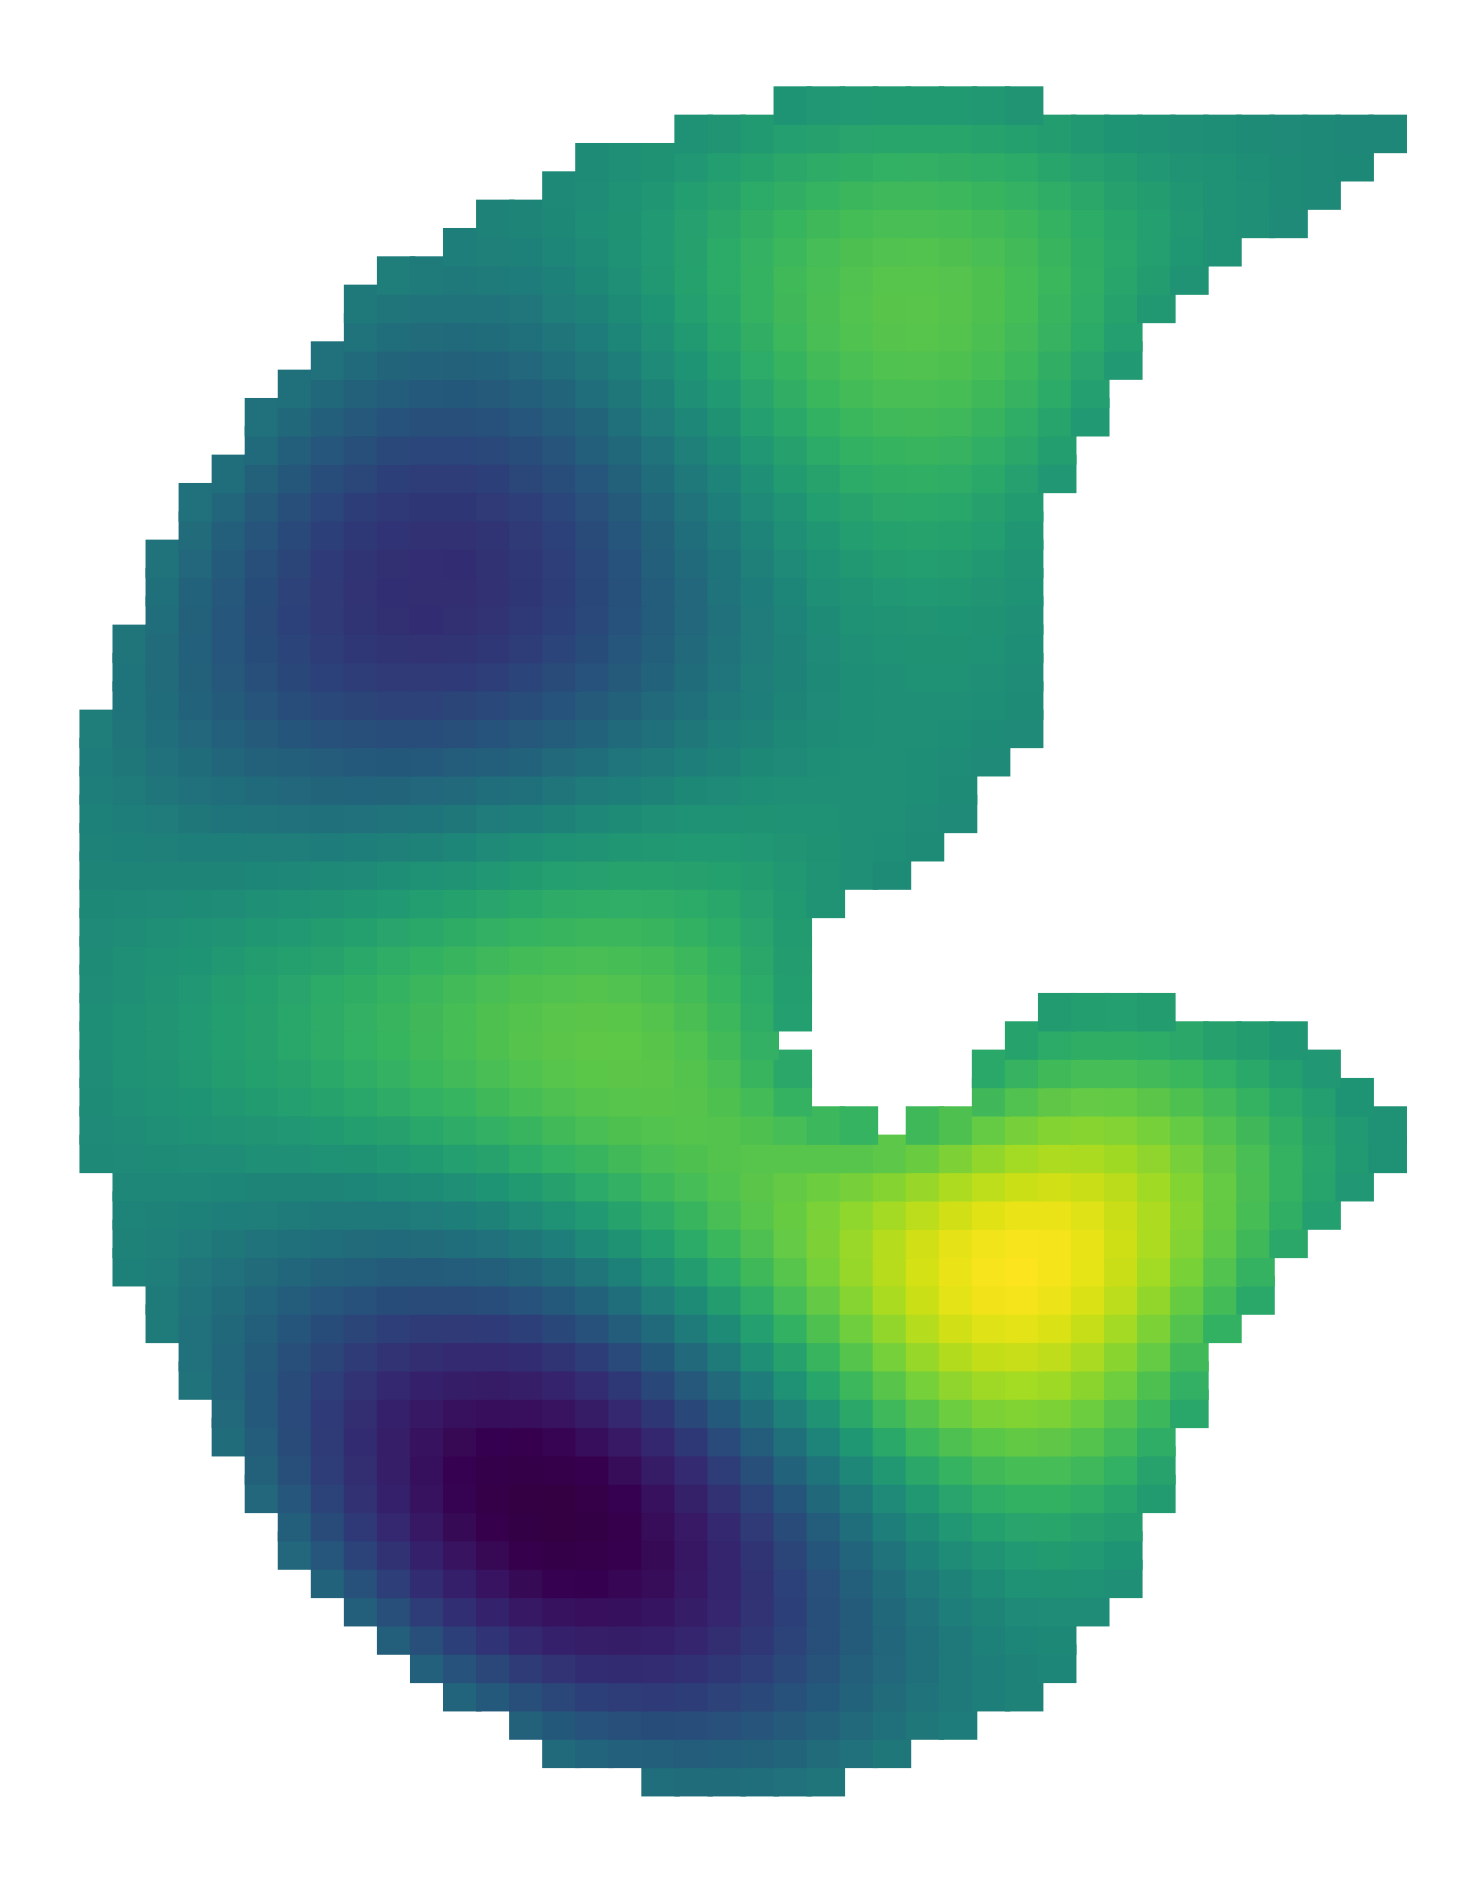
\includegraphics[height=1.5in]{EV4}\\ 

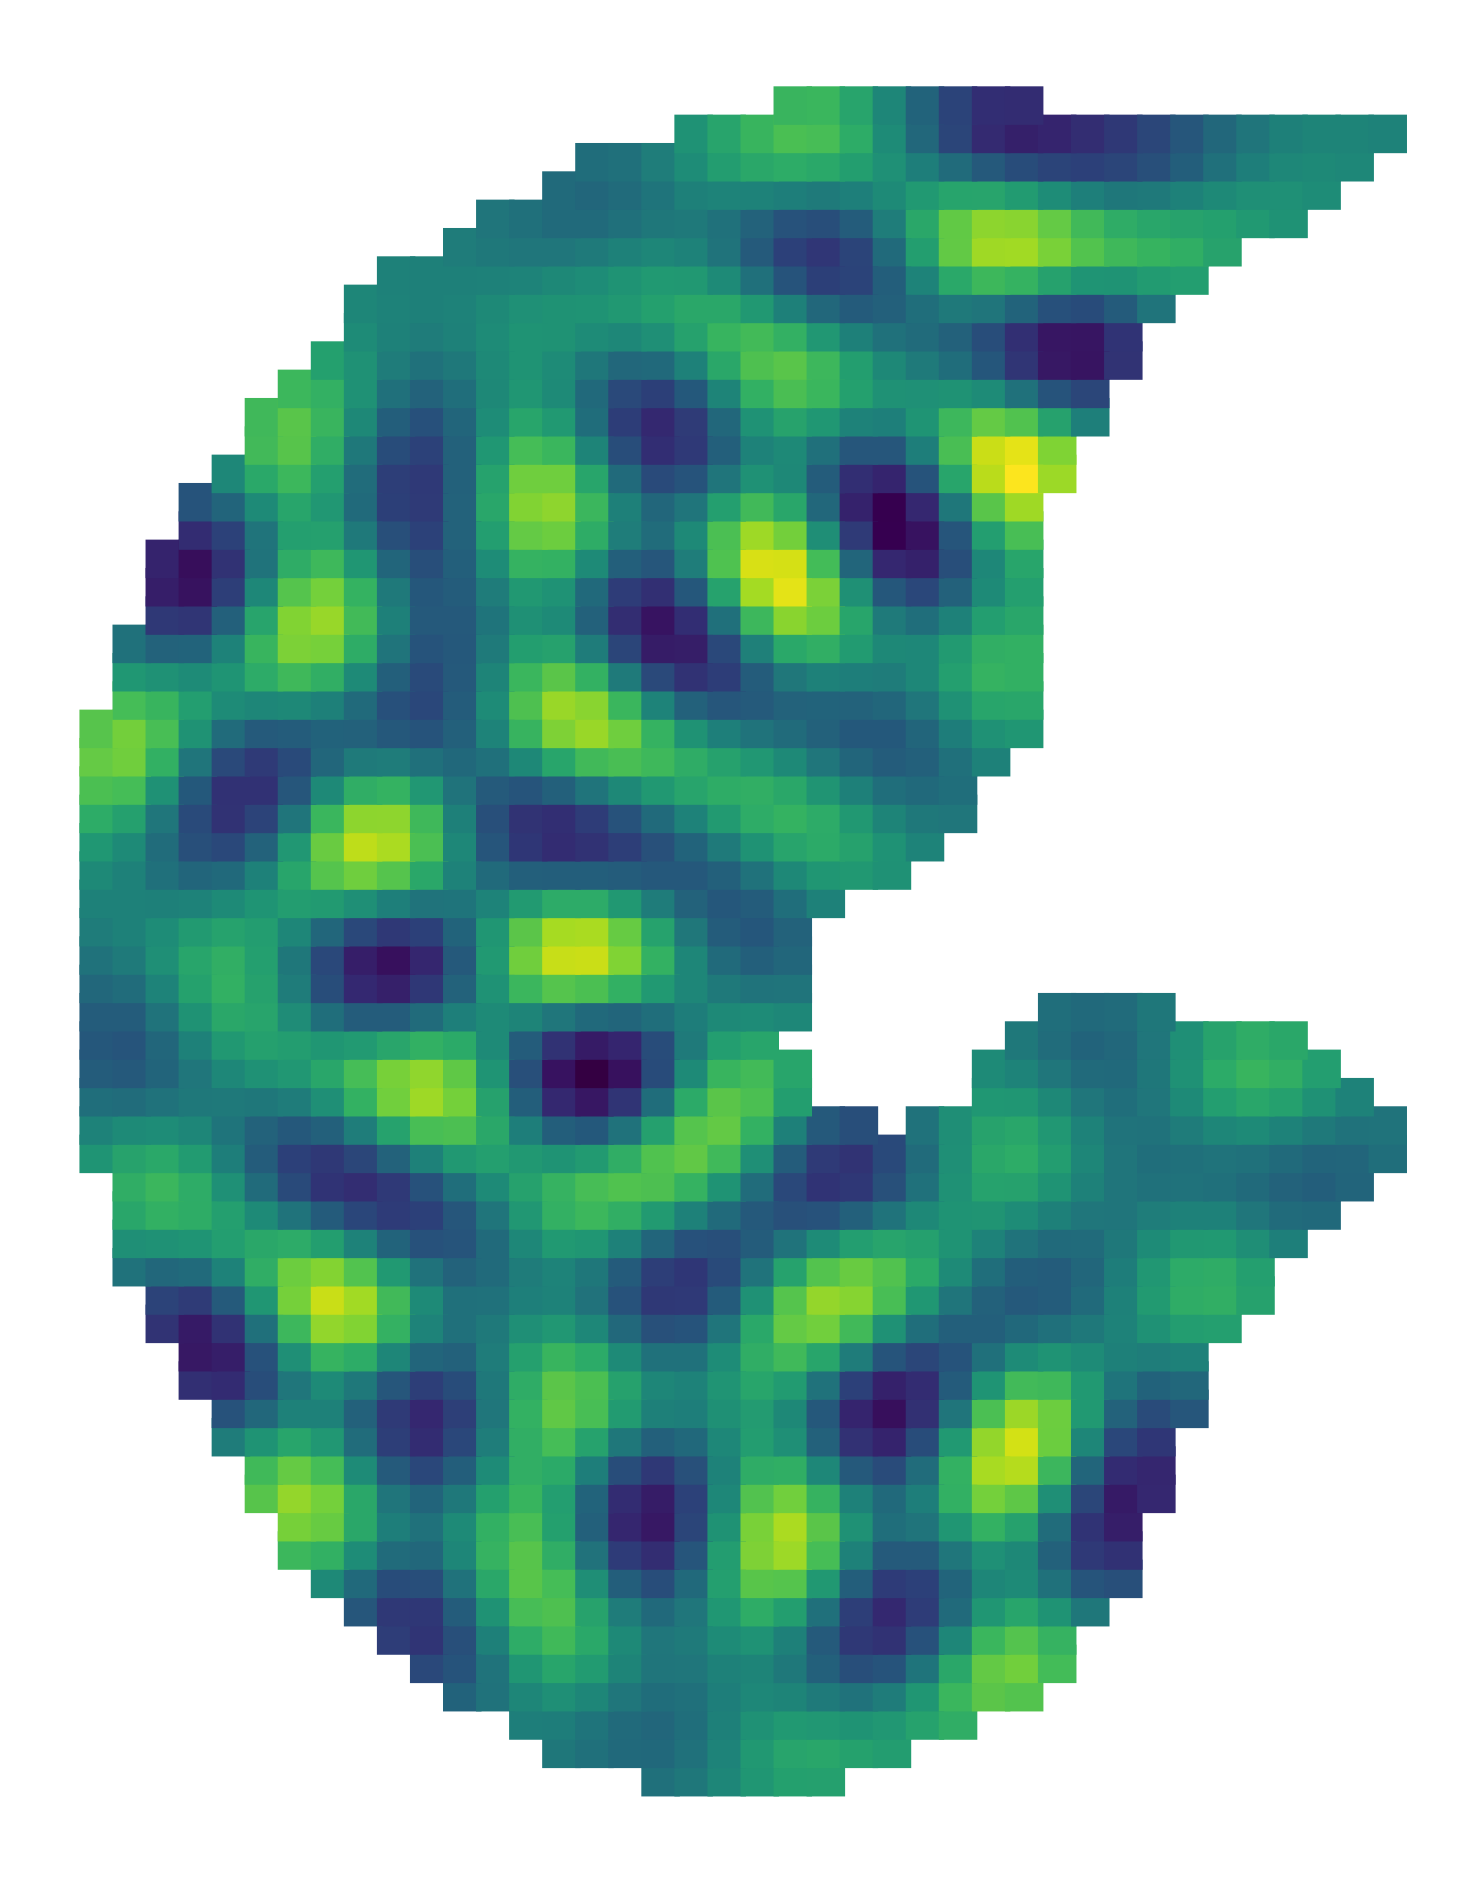
\includegraphics[height=1.5in]{EV100}
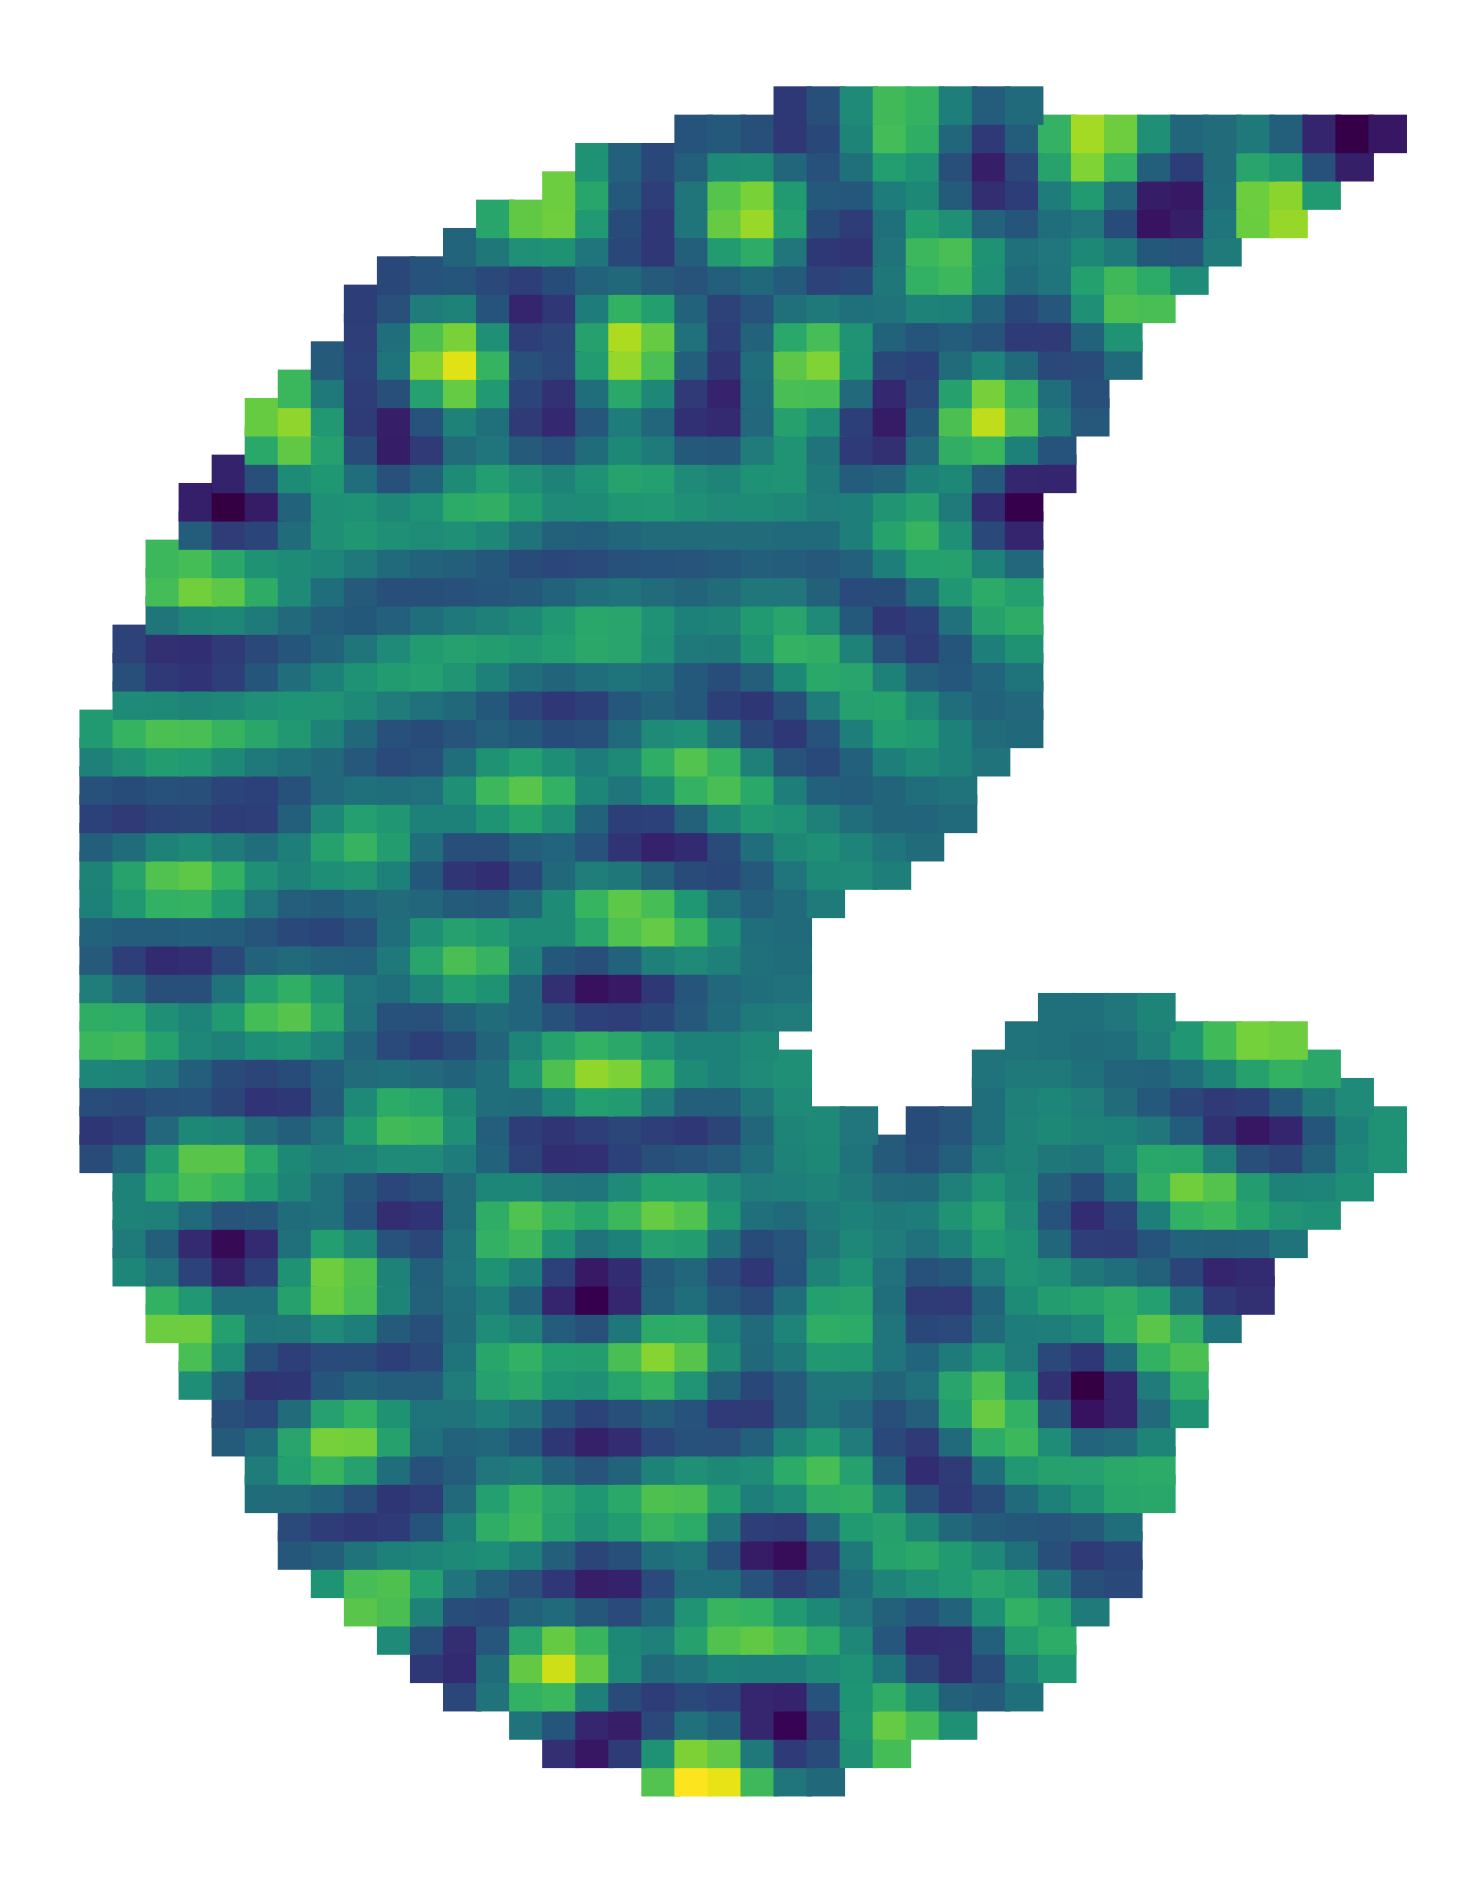
\includegraphics[height=1.5in]{EV200}
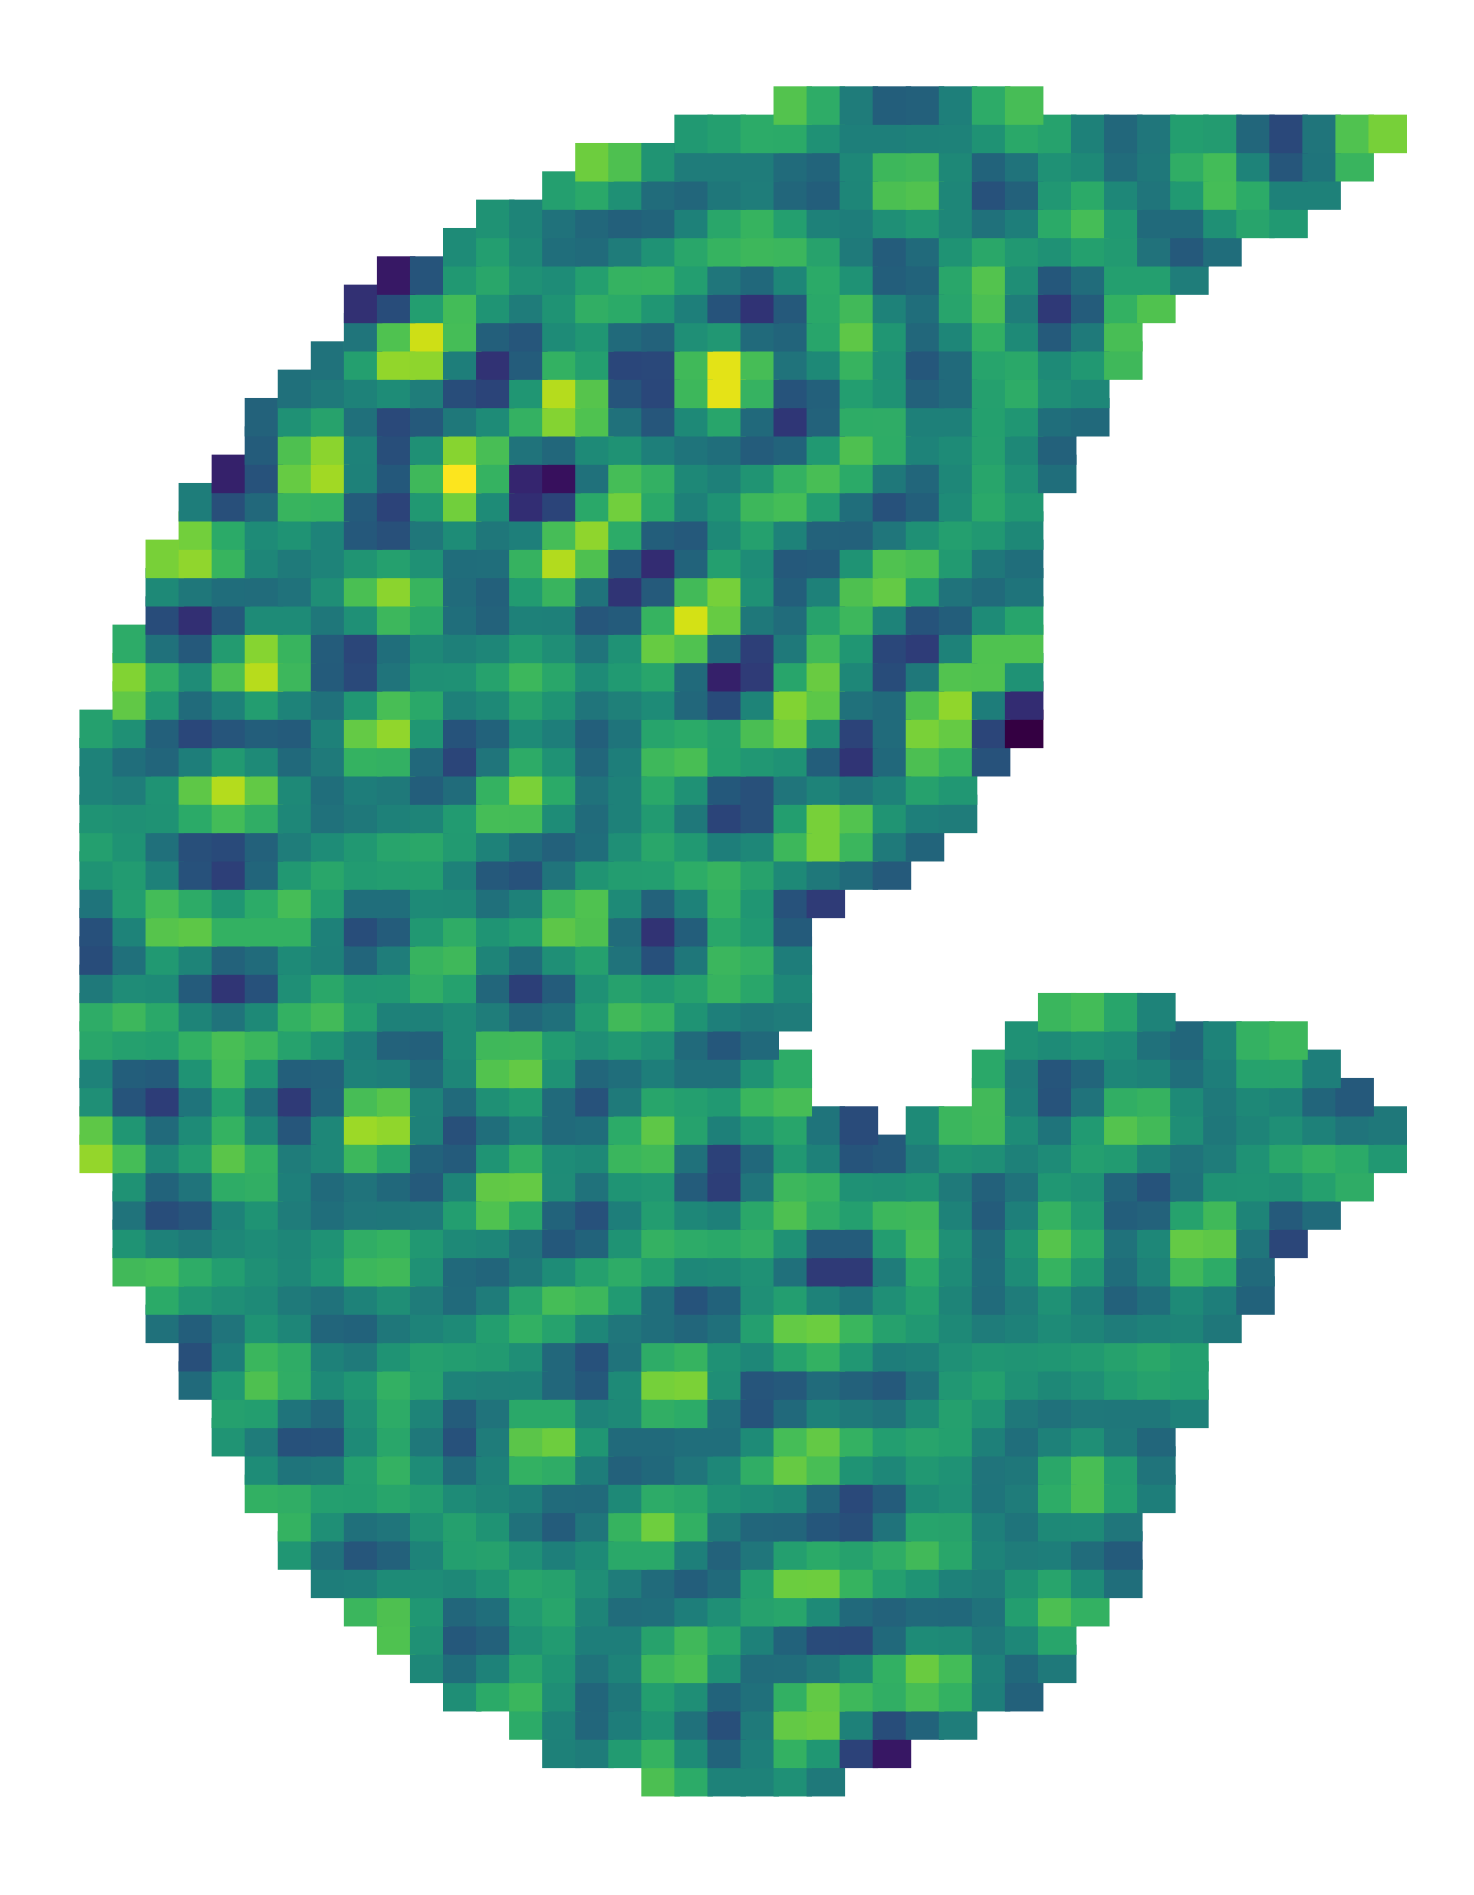
\includegraphics[height=1.5in]{EV300}
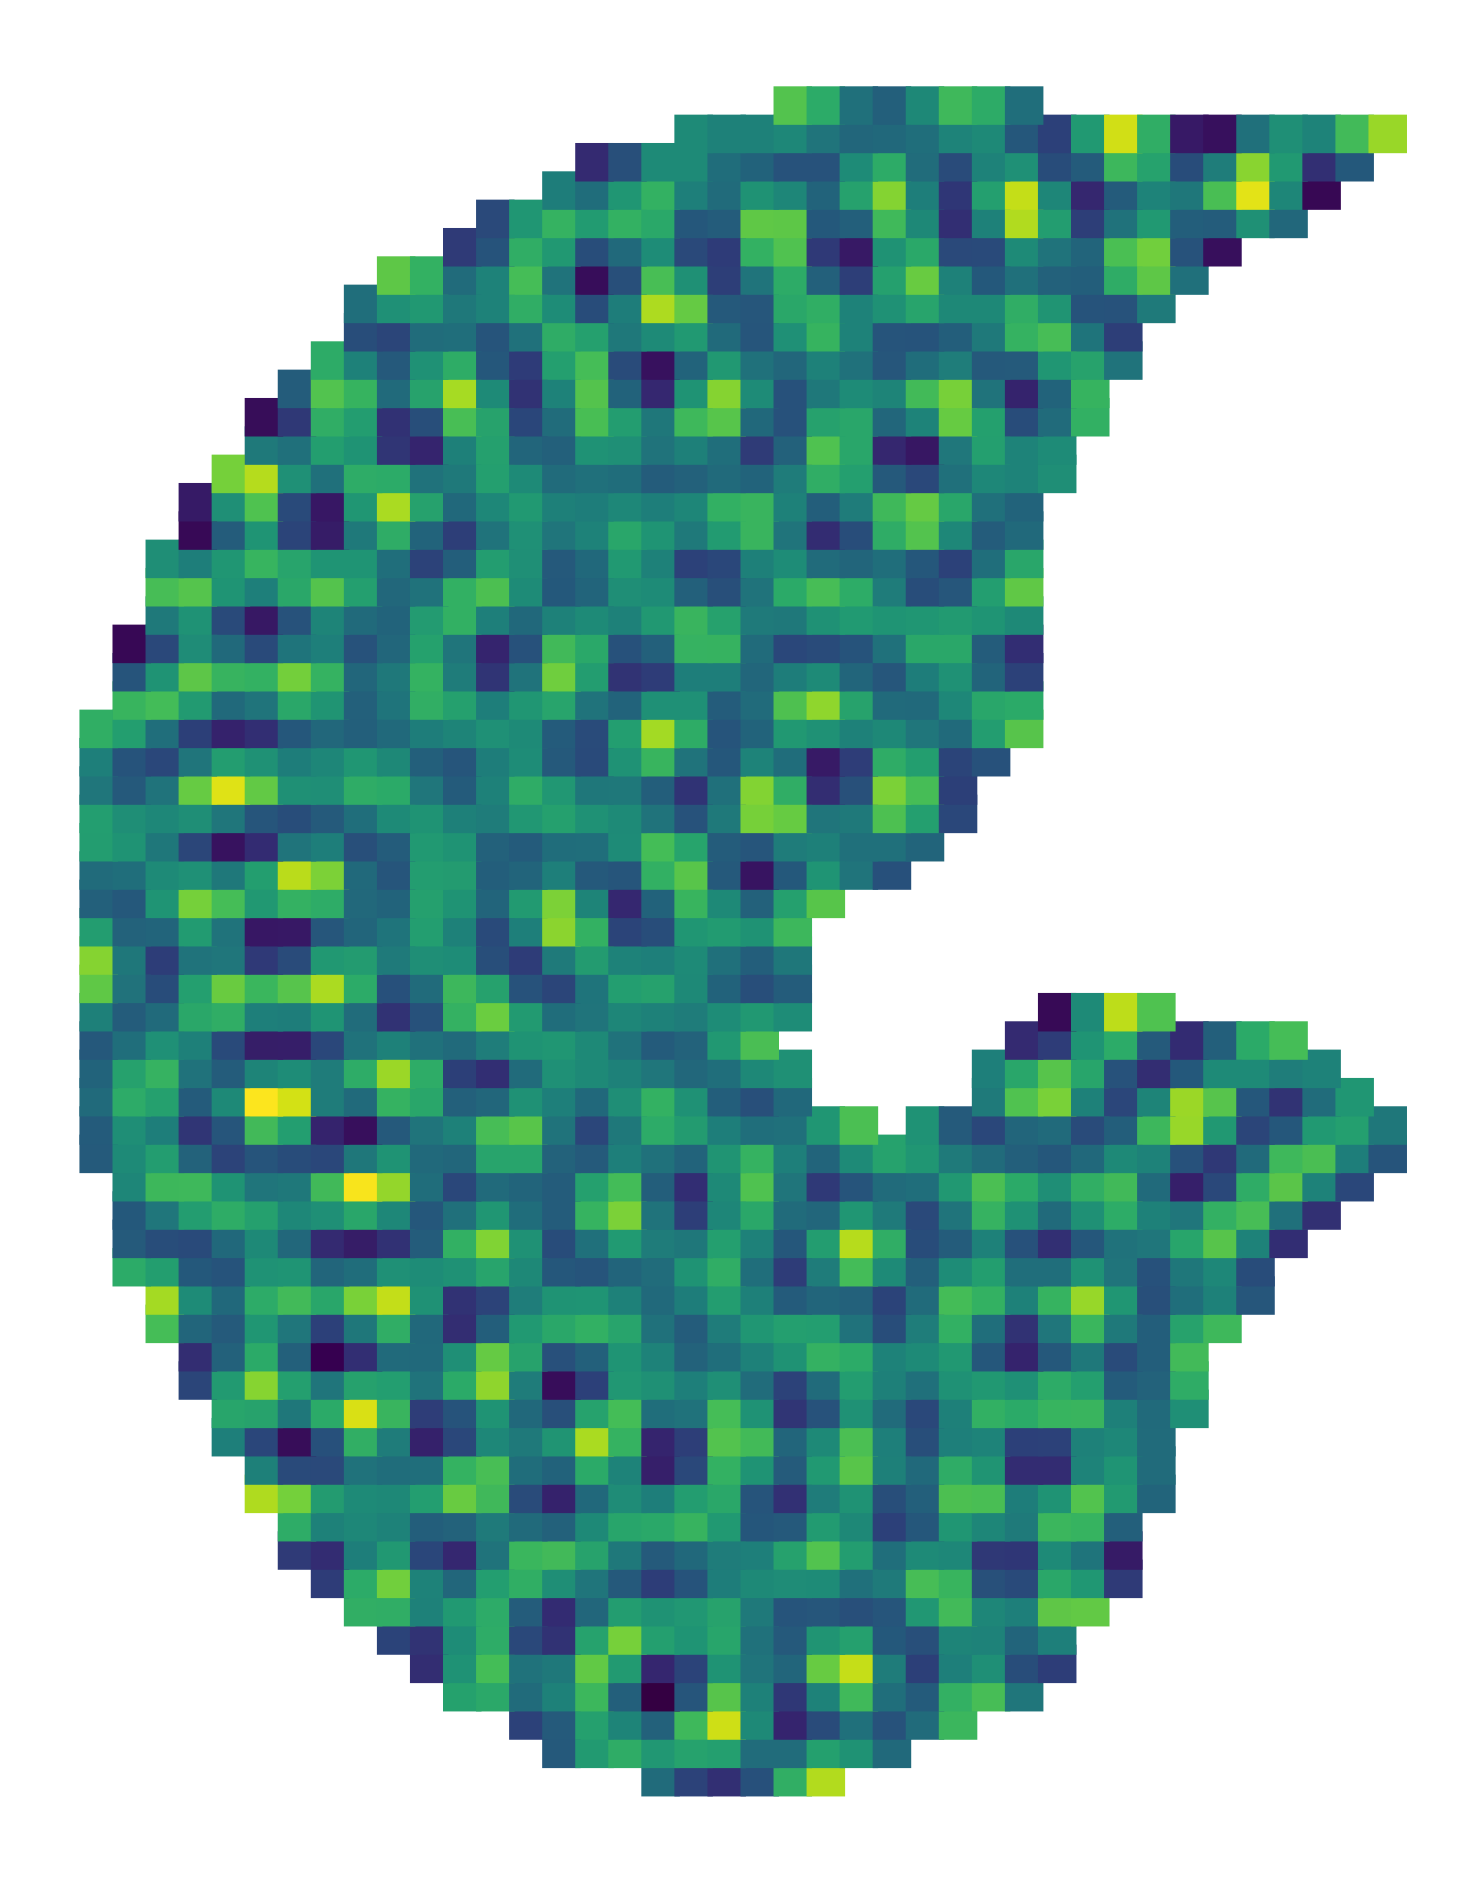
\includegraphics[height=1.5in]{EV397}  
\caption{Moran eigenvectors based on the distance matrix from a 2D axial slice of the lung. The top row corresponds to the 1st - 4th eigenvectors. The bottom row corresponds to the 100th, 200th, 300th, and 397th eigenvectors. }
\label{fig:eigenvectors}
\end{figure}

\subsection{Graph Signal Processing}

\subsection{Links between the two developments}

\subsection{Simulation}
Yue writing up some ideas for the simulations

\subsection{Application to toy example}
\begin{enumerate}
\item{Fit Sarah's model to the toy example}
\item{Predictive model---need to be reminded of what this is}
\item{Use a GSP framework to build network}
\item{Assume spatial correlation network (weight matrix) for an analysis using GSP--what citation do we want to model}
\end{enumerate}

Investigate using different networks to understand how sensitive results are to the specification of the network.

What are 1-2 other features to investigate.

\begin{enumerate}
\item{Fit Sarah's model to GRADS data}
\item{Predictive model---need to be reminded of what this is}
\item{Use a GSP framework to build network on GRADS data}
\item{Assume spatial correlation network (weight matrix) for an analysis using GSP--what citation do we want to model}
\end{enumerate}

\begin{enumerate}
\item{Fit Sarah's model to BioAD data--need to figure out the subsection to use}
\item{Predictive model---need to be reminded of what this is}
\item{Use a GSP framework to build network on BiosAD data}
\item{Assume spatial correlation network (weight matrix) for an analysis using GSP--what citation do we want to model}
\end{enumerate}

\section{Discussion}
We posit(?) that eigen decomposition provides a novel construct for studying factors that influence correlation.

\end{document}

